% begin module tangent-line-power-rule
\begin{frame}
\begin{example}[Calculating the tangent line using the Power Rule]
Find an equation for the tangent line to the cubic $y = \sqrt[3]{x}$ at the point $P = (1,1)$.

\begin{columns}[c]
\column{.4\textwidth}
\psset{xunit=0.8cm, yunit=0.8cm}

\begin{pspicture}(-3, -3)(3.1,3.1)
\psframe*[linecolor=white](-3,-3)(3.1,3.1)
\tiny
\psaxes[labels=none]{<->}(0,0)(-3,-3)(3,3)
\fcLabels{3}{3}
%Function formula: (x)^{1/3}
\psplot[linecolor=red, plotpoints=1000]{0}{3}{x 0.333333 exp }
\psplot[linecolor=red, plotpoints=1000]{-3}{0}{x -1 mul 0.333333 exp -1 mul }
\rput[t](-1,-1.1){$y=\sqrt[3]{x}$}
\rput[tl](1,0.9){$(1,1)$}
\uncover<7->{
\psline[linecolor=blue](-3, -0.33333)(3, 1.666667)
\rput[b](-1,1){$y=\frac{1}{3}x+\frac{2}3$}
}
\fcFullDot{1}{1}
\end{pspicture}
%\only<handout:0| -6>{%
%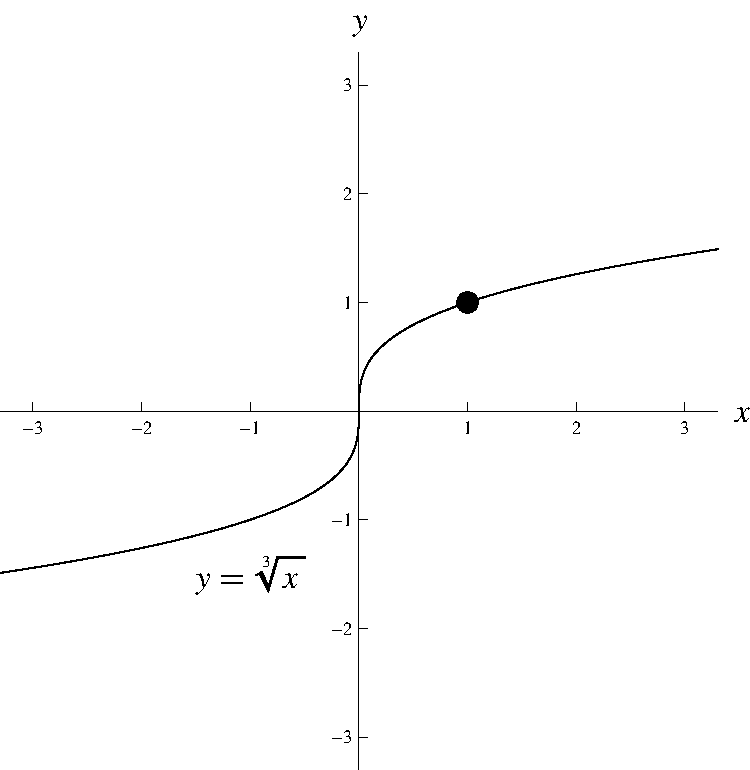
\includegraphics[width=4.5cm]{derivatives/pictures/tangent-line-power-rulea.pdf}%
%}%
%\only<7->{%
%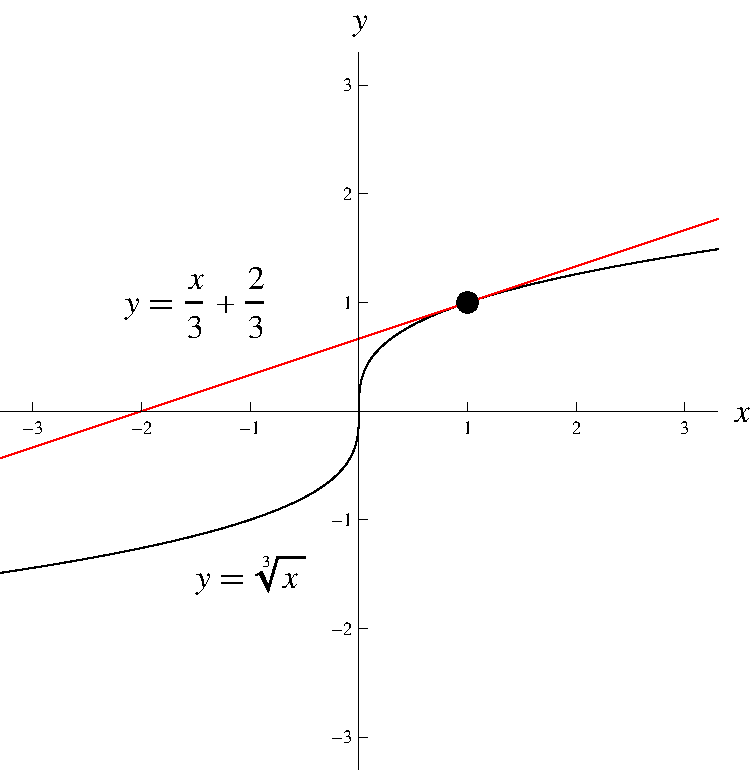
\includegraphics[width=4.5cm]{derivatives/pictures/tangent-line-power-ruleb.pdf}%
%}%
\column{.6\textwidth}
\uncover<2->{%
Here $a = 1$ and $f(x) = \sqrt[3]{x}=x^{\frac{1}{3}}$.
}%
\abovedisplayskip=0pt
\belowdisplayskip=0pt
\abovedisplayshortskip=0pt
\belowdisplayshortskip=0pt

\begin{align*}
\uncover<3->{f'(x)} & \uncover<3->{ = } %
\uncover<3->{\frac{1}{3}x^{\frac{1}{3} - 1} }\\
&\uncover<4->{=} %
\uncover<4->{ \frac{1}{3}x^{\frac{-2}{3} } } \\
&\uncover<5->{ =  } %
\uncover<5->{ \frac{1}{3\sqrt[3]{x^2}}.}\\
\uncover<6->{f'(1)} & \uncover<6->{ =  } %
\uncover<6->{\frac{1}{3}.} \\
\end{align*}
\uncover<7->{
Point-slope form: $y - 1 = \frac{1}{3}(x - 1)$, or $y = \frac{1}{3}x  +\frac{2}{3}$.
}
\end{columns}
\end{example}
\end{frame}
% end module tangent-line-power-rule
